% !Mode:: "TeX:UTF-8"%確保文檔utf-8編碼
%新加入的命令如下: reduline showendnotes 
%新加入的环境如下:solution solutionorbox solutionorlines solutionordottedlines

\documentclass[12pt,twoside]{exam}
\newlength{\textpt}
\setlength{\textpt}{12pt}

\usepackage{teachingplan}

%写上答案或者不写上答案%
\printanswers  


%讲知识点然后测试,测试通过继续下一个知识点。不通过给予小提示,然后继续测试,如果通过那么通过,如果还是不会做,那么继续讲解知识点,并讲解这个题目,然后重新给出一个题目重新测试。

%如果有精力,后面再准备一套中考真题。

%\excludecomment{knowledge}
\includecomment{knowledge}
%\excludecomment{Aquestions}
\includecomment{Aquestions}

\CenterWallPaper{1}{教案模板-2.pdf}

\newcommand{\keti}{临时测评}
\newcommand{\zhongdian}{1.运动的描述 2.质量和密度 \\3.力和运动 4.压强}
\firstpageheader{}{}{\today}
\begin{document}
\ThisCenterWallPaper{1}{教案模板-1.pdf}
\vspace*{70pt}
\keti \par
\zhongdian \par
\begin{knowledge}
\section{临时测评}
\begin{questions}
\question
长度的国际单位是\answerline*[米],常用的国际单位及其符号有:千米(km)、分米(\answerline*[dm]) 、厘米(cm)、毫米(\answerline*[mm])、微米(\si{\micro m}
)、纳米(\answerline*[nm])。

\question
使用刻度尺注意事项:
\begin{enumerate}
\item[①] 注意刻度标尺的零刻度线、最小\answerline*[分度值]和量程。
\item[②] 测量时尺要沿着所测长度,尽量靠近被测物体,不用磨损的零刻度线。
\item[③] 读数时视线要与尺面\answerline*[垂直],在精确测量时要\dotuline{估读}到分度值的下一位。
\item[④] “记”,测量值由数字和\answerline*[单位]组成,最末一位是\answerline*[估读]值,包括估读值在内的测量值称为有效数字。
\end{enumerate}


\question
\textbf{(2013广西南宁,1,2分) } 2012年11月23日,国产歼-15舰载机首次在航空母舰“辽宁号”上成功起降。如图所示,飞机起飞时,若说该飞机上的飞行员是静止的,所选的参照物是(\answerline*[B])

\begin{oneparchoices}
\choice 航母 
\choice 该飞行员驾驶的飞机
\choice 海水
\choice 航母上的工作人员
\end{oneparchoices}

\begin{linefig}[0.8]{2013广西南宁1}
\end{linefig}



\question
甲、乙两辆汽车在水平路面上同时向东行驶,路程-时间图像如下图所示,则甲车的速度是\answerline*[15]$m/s$;两车行驶过程中,若以甲车为参照物,乙车向\answerline*[西]运动。

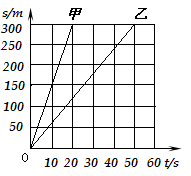
\includegraphics[scale=1]{figures/图片11.png} 


\question
如下图所示,量筒的直径$d$为\answerline*[1.20]$cm$。

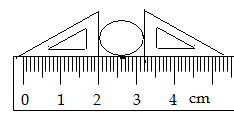
\includegraphics[scale=1]{figures/图片12.png} 

\question
\textbf{(2011北京,1,2分)}在国际单位制中,质量的单位是(\answerline*[A])

\begin{oneparchoices}
\choice 千克
\choice 牛顿
\choice 帕斯卡
\choice 焦耳
\end{oneparchoices}

\question
\textbf{(2013广西南宁,16,2分)}利用橡皮擦将纸上的字擦掉之后,橡皮擦的质量\answerline*[变小],密度\answerline*[不变](以上两空选填“变小”、“变大”、“不变”)。

\question
\textbf{(2013湖南长沙,30,4分)}浏阳腐乳以其口感细腻、味道纯正而远近闻名,深受广大消费者喜爱。现测得一块腐乳质量约为10g,体积约8\si{cm^3},则其密度为\answerline*[1.25]\si{g/cm^3}。若吃掉一半,剩余部分的密度将\answerline*[不变]。

\question
\textbf{(2013河北,15,2分)}第一位提出“物体的运动并不需要力来维持”的物理学家是(\answerline*[A])

\begin{oneparchoices}
\choice 伽利略
\choice 奥斯特
\choice 帕斯卡
\choice 阿基米德
\end{oneparchoices}


\question
力的三要素是力的\answerline*[大小],\answerline*[方向],\answerline*[作用点]。只要有一个要素发生变化,力的作用效果就会改变。

\question
\textbf{(2012上海,17,3分)}重为4牛的球体静止在水平地面上,用力的图示法在图中画出它受到的重力$G$。
\begin{linefig}[0.5]{2012上海17-1}
\end{linefig}



\question
当你轻轻推一个箱子是,箱子不动,这个时候箱子的受力是推力\answerline*[等于]摩擦力(此时的摩擦力是\textbf{静摩擦力})。而当你再加把劲推动箱子时,箱子还是不动,这个时候还有推力等于摩擦力,而且此时的摩擦力是\answerline*[大于]之前轻轻推时箱子所受到的摩擦力的。当你再加把劲的时候箱子终于推动了,这个时候摩擦力变成了\textbf{滑动摩擦力}。

滑动摩擦力既跟作用在物体表面的压力有关,又跟接触面的粗糙程度有关。压力越大,则滑动摩擦力\answerline*[越大],接触面越粗糙,则滑动摩擦力\answerline*[越大]。


\question
在一些公共汽车上配备逃生锤,遇到紧急情况时,乘客可以用逃生锤打破玻璃逃生,为了更容易打破玻璃,逃生锤外形应选择下面的(\answerline*[C])
\begin{choices}
\begin{multicols}{4}
\choice 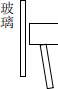
\includegraphics[scale=1]{figures/图片1-1.png} 
\columnbreak
\choice 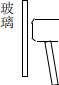
\includegraphics[scale=1]{figures/图片1-2.png} 
\columnbreak
\choice 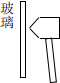
\includegraphics[scale=1]{figures/图片1-3.png} 
\columnbreak
\choice 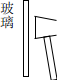
\includegraphics[scale=1]{figures/图片1-4.png} 
\end{multicols}
\end{choices}


\question
测定大气压强数值的是托里拆利(意大利科学家)。托里拆利管倾斜后,水银柱高度\answerline*[不变],长度\answerline*[变长]。


\question
如下图所示,在倒置的透明漏斗里放置一个乒乓球,用手指托住乒乓球,松手后,乒乓球受重力作用将下落;若向倒置的漏斗用力吹气再松手时,乒乓球不但没有被吹下去,反而被“吸”住了。这是因为乒乓球上方空气的流速\answerline*[大于] (填“大于”、“小于”或“等于”)其下方空气的流速,依据流速越大的位置压强越\answerline*[小]的原理,乒乓球受压强差的作用而不下落。

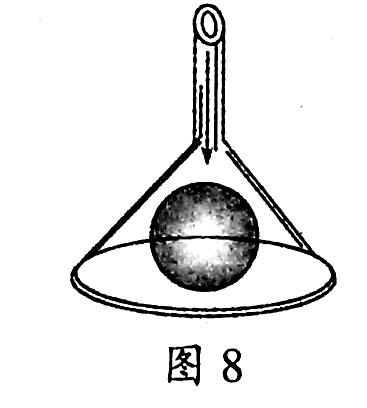
\includegraphics[scale=0.2]{figures/图片10.jpg} 



\end{questions}
\end{knowledge}









%
\ThisCenterWallPaper{1}{教案模板-3.pdf}

\end{document}



